\section{Foundation\label{sec:foundation}}
In this chapter, the basic concepts fundamental to understanding the subject of the thesis will be explained. This will allow a better understanding of the following chapters and the proposed solutions. Firstly, the foundations of systems engineering will be presented. Then the notions of CAD, CAE, and “Expert System” will be explained. This will be followed by an introduction to semantic technologies. This will be followed by an analysis of the use of semantic technologies in the field of systems engineering. 

\subsection{System Engineering \label{sec:sysen}}
Systems engineering is a multidisciplinary approach to the design, implementation and management of complex systems throughout their life cycle (see Figure). It embraces a holistic perspective that takes into account the interactions and interdependencies between different components in order to achieve optimal performance and functionality. Systems engineering deals with work processes, optimisation methods and risk management tools in projects. Systems engineering ensures that all likely aspects of a project or system are considered and integrated as a whole. In the context of the automotive industry, where complex systems and simulations play a central role, the application of systems engineering principles becomes paramount.

\subsubsection{Core Concepts}
    The key principles of systems engineering are as follows:
    \begin{itemize}
      \item Requirements engineering: this phase consists of determining and documenting the needs and constraints that the system must satisfy. In the context of simulation configuration, understanding requirements is crucial to accurately model and simulate real-world automotive scenarios.
      
      \item System design: this phase involves transforming the requirements into a system plan. It involves assigning functions to components, taking into account factors such as efficiency, reliability, and maintainability. For simulation configuration, this step is essential to create a framework that aligns with the specific attributes of automotive simulations.
      
      \item Integration and testing: Systems engineering emphasizes the importance of rigorous testing and integration to ensure that all components work perfectly together. This is particularly relevant in the context of simulation configuration, where the accuracy and reliability of results depend on the effective integration of different simulation parameters.
      
      \item Lifecycle management: Systems engineering goes beyond the initial design and implementation phases. It involves continuous monitoring, maintenance and adaptation to changing requirements throughout the system's lifecycle. This perspective is crucial to the longevity and adaptability of simulation configurations in the dynamic automotive landscape.

    \end{itemize}

    
\subsubsection{V-Model}
The V-model illustrates systems development by highlighting the verification and validation stages. A graphical representation of this model is shown in Figure \ref{fig:v-model}. The system specification and detailed software design are presented on the left-hand side of the “V”, along with the steps leading to implementation. The steps mentioned on the left-hand side must be verified and validated on the right-hand side of the “V”. It also includes the integration of systems and software. Each step on the left is directly linked to a test step. Once the first stage has been successfully completed, the next stage begins.\\

\begin{figure}[H]
    \centering
    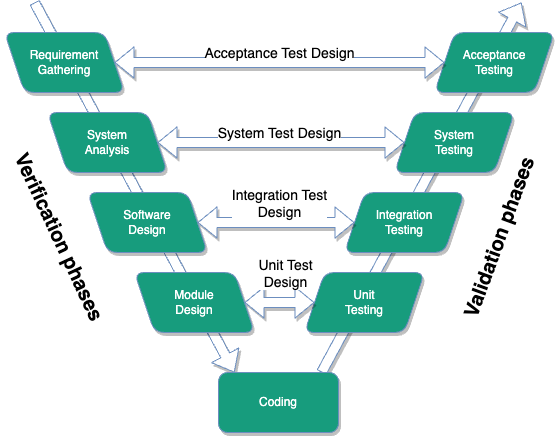
\includegraphics[scale=0.6]{images/V-Model.png}
    \caption{\label{fig:v-model} V-Model }
\end{figure}

With the evolution of technology, many software applications exist to cover these different stages more effectively. 

\subsection{Computer Aided Engineering and Simulation}
CAE, also known as digital engineering or computer-aided engineering, brings together all the digital and software resources usually used by engineers to design, simulate and validate new products and industrial processes using sophisticated algorithms. CAE tools enable the physical properties of a product to be tested and simulated, so that it can be optimized on the basis of the results of a numerical analysis.

    \subsubsection{Simulation-driven design}
    Typically, CEA involves pre-processing, solving and post-processing stages. During the pre-processing phase, engineers model the system, the physical properties of the design, and the operational environment in the form of applied constraints or loads. In order to correctly configure the resulting simulations, it is crucial that this modelling incorporates all parts of the environment to which the product will be exposed (including forces, temperatures, etc.).  The quality of the simulation is largely determined by the accuracy of the conditions to which the product will be exposed. The model is then solved using simulations before the results are presented for review during post-processing. \\

    Whereas physical prototyping takes days or even weeks, simulations take just a few hours at most. Although physical prototyping is unavoidable, simulations can help reduce the number of prototypes needed before production.\\
    
    Figure \ref{fig:v-model-sim} shows the different types of simulations and tests throughout the “V” model presented above. Initial design and simulation of CAD geometry under appropriate conditions is the CEA's standard workflow. Based on the results of the simulation, the design is improved. This process may need to be repeated until the product requirements are met and virtually confirmed. If there are differences in behavior between the digital prototype and expectations, the CAD model or input data can be adjusted. This process speeds up product development because there is no need to create physical prototypes in the early stages of development.

    \begin{figure}[h]
        \centering
        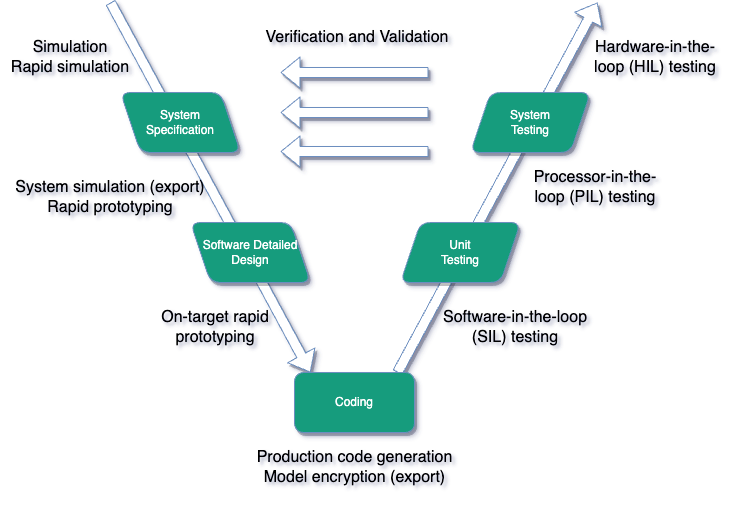
\includegraphics[scale=0.6]{images/Foundation-V-Model-Sim.drawio.png}
        \caption{\label{fig:v-model-sim} V-Model with simulations }
    \end{figure}


    \subsubsection{Advantages}
    One of the main advantages of this approach is that it only takes a few hours, whereas it takes several days or even weeks to build and test physical prototypes. Of course, there will always be a need to build a physical prototype at some point, but CAD greatly reduces the number of prototypes required. The use of CAD and the resulting reduction in the need for physical prototypes means that product development costs and time can be reduced, while guaranteeing better product quality.\\

    The benefits of CAE include
    \begin{itemize}
        \item Saving money: Compared to building several real prototypes, using computer simulations to evaluate designs is less expensive.
        \item Time savings: using CAE design tools means that designs can be created faster and more efficiently.
        \item Simple design editing: With CAE, editing a design is quick and easy. This allows you to correct errors and make changes to your design, enabling problems to be solved quickly and further savings to be made.
        \item Fewer errors: Compared with manual design, CAD can reduce the likelihood of errors.
        \item Less work: since CAE software automates a large part of the operation, designing various models requires less work.
        \item Less duplication of work: As the computer code is reusable, it is not necessary to perform the same activities several times. In addition, separate code segments can be duplicated and used during the design process.
        \item Easy to share: CAE design files can be easily saved and exchanged.
        \item Greater accuracy: CAD software is more accurate than manual design, allowing you to work more precisely and achieve better results.
        \item Better decision-making: Performance impacts can guide design choices, and these impacts can be assessed early in the development phase, when it is cheaper and simpler to make changes to the design.
    \end{itemize}

    \subsubsection{Inconvenient}
    While CAD has many advantages, others argue that it is difficult to control the design of increasingly complicated components, as the correct results only appear later in the product design cycle. To overcome this difficulty, CAE's software suppliers are constantly creating new tools and streamlining existing procedures. In addition, CAD can have the following disadvantages:

    \begin{itemize}
        \item Hardware Failure: A computer breakdown might result in job loss.
        \item Security: Work might be subject to hackers or viruses.
        \item Employee Competencies: Learning how to utilize the CAE program may require some training.
        \item System Expense: Purchasing new systems can be expensive.
        \item Updates: Recurrent system updates may be required.
    \end{itemize}

\subsection{Expert System\label{subsec:exp-sys}}
An expert system in artificial intelligence is a computer program that simulates the decision-making process of a human expert[]. It possesses knowledge in a given domain, extracted from the knowledge of experts in that domain.  Rather than using traditional procedural code, expert systems are designed to deal with complex questions posed by the user by reasoning from bodies of knowledge. The 1970s saw the development of the first expert systems, which came into widespread use in the 1980s[]. They were one of the first applications of artificial intelligence (AI) software to achieve real success[]. \\

Figure \ref{fig:es-archi} shows the architecture of an expert system. An expert system consists of two subsystems: the knowledge base and the inference engine. Rules and information are represented in the knowledge base. To deduce new facts, the inference engine applies the rules to the known facts. In addition, inference engines can be capable of debugging and explanation.\\

A non-expert user uses this software to gather information, while people who are experts in a given field enter data into the knowledge base. It is widely used in a number of fields, including coding, games, accounting and medical diagnostics. They can guide users and explain how they arrived at a specific recommendation or conclusion.\\

The process of creating an expert system is called 'knowledge engineering', and the people who carry it out are known as knowledge engineers. The main responsibility of the knowledge engineer is to ensure that the computer has all the knowledge it needs to solve a problem. To express the necessary information in the form of a symbolic model in the computer's memory, the knowledge engineer must choose one or more forms (the ontology will be chosen for the purposes of this thesis).\\

\begin{figure}[h]
    \centering
    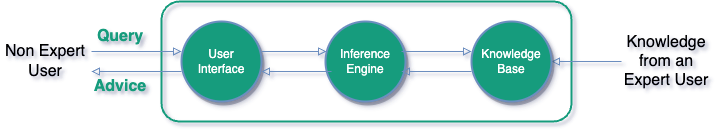
\includegraphics[scale=0.6]{images/Foundation-Architecture_Expert_System.drawio.png}
    \caption{\label{fig:es-archi} Architecture of an Expert System }
\end{figure}

Components of an expert system : 
\begin{itemize}
    \item Knowledge base: Facts and rules are represented here. It is made up of intrinsic facts relevant to the domain, methods, rules for solving problems and knowledge specific to the domain.
    \item Inference engine: this retrieves relevant information from the knowledge base, analyses it, and determines a solution that addresses the user's problem. To deduce new facts, the inference engine extracts rules from its knowledge base and applies them to known facts. In addition, debugging and explanation functions can be added to inference engines.
    \item Learning and knowledge acquisition module: The aim of this part is to enable the expert system to collect and store knowledge from various sources on an ongoing basis.
    \item User interface: Using this module, a non-expert user can communicate with the expert system and work out a solution.
    \item The explanation module helps the expert system to provide the user with a detailed explanation of how it arrived at a certain result.
\end{itemize}


\subsection{Semantic Web\label{sec:semweb}}
The Semantic Web is an expansion of the World Wide Web that intends to enable robots to comprehend and interpret the meaning of content on the internet. It entails encoding data in a way that improves interconnectivity, connecting similar information, and enabling computerized processing. The objective is to improve information retrieval efficiency while also enabling more intelligent online apps and services.\\

In 2001, Tim Berners-Lee coined the term “Semantic Web” to describe the use of semantic technologies in data connectivity [ ]. The World Wide Web Consortium (W3C), founded by Berners-Lee, disseminates and supports a number of technical guidelines for the Semantic Web. “Semantic web technologies allow people to create data shops on the web, build vocabularies and write rules to process data”.\\

Improving the way computers understand data makes it easier to share data and enables it to be processed automatically. As Figure \ref{fig:sem-web-stack} shows, the Web Ontology Language (OWL), SPARQL and Resource Description Framework (RDF) are the main standards on which semantic technology is developing. In contrast, in conventional information technology, meanings are hard-coded into application code and data at the design stage. \\

\begin{figure}[h]
    \centering
    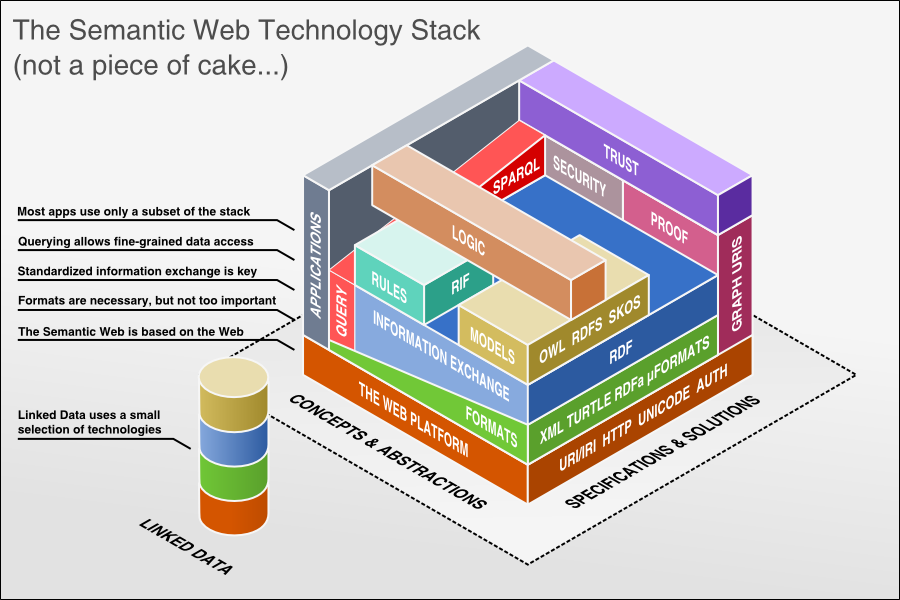
\includegraphics[scale=0.6]{images/foundation-sem-web-tech-stack.png}
    \caption{\label{fig:sem-web-stack} Semantic Web Technologies Stack }
\end{figure}


    \subsubsection{URI and IRI}
        \paragraph{URI}
        A URI is a short string of characters that clearly identifies an abstract or physical resource on the Semantic Web. The use of URIs makes resources available through a number of naming systems and access mechanisms. A URI can be used for location, identification, or both. There are two types of URI: URLs (Uniform Resource Locators) and URNs. A URL is a subset of a URI that indicates the location of a resource and how to retrieve it. A URN, on the other hand, is used to identify an online resource without specifying how it will be retrieved.\\

        Semantic Web resource identifiers can be divided into a base URI and a local name. In serialization, the base URI is often shortened by a prefix defined at the beginning. Figure \ref{fig:uri-example} shows an example of a URI and its decomposition with a prefix.\\

        \begin{figure}[h]
            \centering
            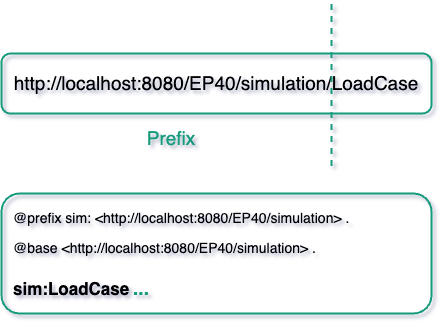
\includegraphics[scale=0.6]{images/Foundation-URI Decomposition.drawio.png}
            \caption{\label{fig:uri-example} Example of URI and decomposition with prefix}
        \end{figure}

        
        \paragraph{IRI}
        The Internationalized Resource Identifier (IRI) is an extension of the URI that adapts to a global character set, whereas the URI is limited to ASCII and has far fewer characters. IRIs enable the representation and communication of data-related knowledge in several languages. IRIs can be transformed into URIs using percentage encoding, enabling backward compatibility.


    \subsubsection{RDF}
    RDF is a resource description framework developed by W3C. It is used in particular on the World Wide Web for data exchange. The RDF data model allows data resources to be uniquely recognized and linked to other data resources for reading, analysis and action. 

    RDF [ ] introduces several fundamental Semantic Web terms:

    \begin{itemize}
        \item A resource is anything that can be characterized by an RDF declaration. URIs ensure that resources are always uniquely named. Any physical thing or notion can be represented by a URI, allowing RDF to be used to describe different types of domains.
        \item Description:
        \item Framework:
        \item A “thing” is either an individual object, called an instance, or a definition of a type of thing, called a class. 
        \item A schema is an abstract description of a set of objects. It consists of a hierarchical taxonomy that describes how the elements of the domain are classified. In RDF, schemas are also known as terminology boxes (Tboxes). 
        \item A property is an attribute, feature, characteristic or connection that facilitates the description of a URI. In the RDF architecture, a property is also represented in the form of a URI. It always has a precise meaning and determines the type of resource it can describe, known as the property domain, as well as the permitted values. It can also specify how it relates to other attributes. 
        \item “Axioms” are property declarations for schema classes, often known as Role Boxes (Rbox) in RDF. They define the relationships between classes.
    \end{itemize}

    RDF is a model based on “Triples”. Triples are built around subject-predicate-object relationships, and are the most common type of axiom. The predicate is a property or a relation; the subject is a “thing”. When the object is a thing, the property is called an object property. If the object is a literal, such as a character, integer or string, the property is called a data property. Once a triplet has been defined, it is referred to as a statement.\\

    Take, for example, this basic English sentence: “Germany is in Europe”. Table\ref{tab:rdf-example} shows how the sentence can be divided syntactically. If this statement were to be expressed visually, this could be done using the following directed graph, shown in Figure \ref{fig:rdf-example}.\\
    
    \begin{table}[h]
        \centering
	    \rowcolors{2}{teal!10}{white}
	    \begin{tabular}{ | m{4cm} | m{4cm} | m{4cm} | }
            \hline
            \rowcolor{teal!30} Subject & Predicate & Object \\
            
            \hline
            Germany  & is in & Europe\\
            
            \hline
        \end{tabular}
        \caption{\label{tab:rdf-example} RDF Syntactic division}
        \end{table}
        
    \begin{figure}[h]
        \centering
        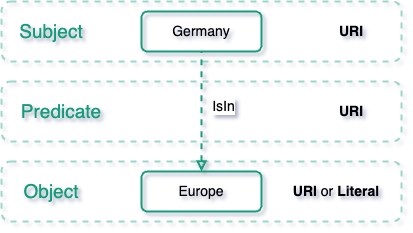
\includegraphics[scale=0.6]{images/Foundation-RDF Example.drawio.png}
        \caption{\label{fig:rdf-example}  RDF Graphical representation}
    \end{figure}

    RDF uses the same techniques to demonstrate the links between subjects and objects. However, as explained earlier, to represent resources and features accurately on the web, they need to be assigned a unique URI. To demonstrate the representation of the above example sentence as a triple, the URIs of the resources and attributes are assumed to be those shown in Table\ref{tab:rdf-example-uri}.
    
    \begin{table}[h]
        \centering
	    {\rowcolors{2}{teal!10}{white}
	    \begin{tabular}{ | m{2.5cm} | m{2.5cm} | c | }
            \hline
            \rowcolor{teal!30} Entity & Role & URI \\
            
            \hline
            Germany  & Subject & $<http://example/resource/Germany>$\\
            
            \hline
            is in  & Predicate & $<http://example/resource/isIn>$\\
            
            \hline
            Europe  & Object & $<http://example/resource/Europe>$\\
            
            \hline
        \end{tabular}}
        \caption{\label{tab:rdf-example-uri} Example of URI Scheme}
    \end{table}

    \subsubsection{Linked Data Principles}
    Linked data is a way of representing and distributing structured data on the web. Data generated and structured according to Linked Data principles is machine-readable and connected to other data on the web. It uses conventional web technologies such as HTTP, RDF and URI, but not only does it provide human-readable data via web pages, it also makes it machine-readable [ ]. Linked data allows concepts, elements, events, people, places, etc. to be organized and linked together. There are many platforms on the web that make available a large amount of linked data and the relationships between them. These include WikiData, DBpedia and Linked Open Vocabularies (LOV).\\

    Tim Berners-Lee, the initiator and defender of the Semantic Web and linked data, established the four design principles of linked data back in 2006.
    \begin{enumerate}
        \item Use URIs to name objects.
        \item Use HTTP URIs to provide useful information. 
        \item Use open standards such as RDF and SPARQL to provide meaningful information about what a name indicates when searched. 
        \item Include connections to other URIs to allow them to find new information. 
    \end{enumerate}

    The more data is represented as linked data on the web, the greater the possibility of linking it to other linked data sources. For example, if a resource represented by a URI in one data source is discovered in an existing linked data source (e.g., WikiData or DBpedia), it can be connected to a property such as “owl:sameAs” to extract further metadata and investigate links to other data resources [ ].\\

    \subsubsection{Ontology}
    In the field of philosophy, ontology is a discipline that studies existence, the way in which knowledge, language, and perception are related to the nature of reality. It is concerned with the question of what entities exist and how they can be classified, ordered hierarchically and discriminated against. \\
    Since the mid-1970s, AI researchers have realized that knowledge engineering is essential for developing large and powerful AI systems[ ]. AI researchers suggested that they could develop new ontologies as computational models to enable certain types of automated reasoning, but their efforts were only moderately successful. In the 1980s, the AI community began using the term ontology to describe both a theory of a modelled world and a component of knowledge-based systems [ ].\\
    An ontology captures the structure of a domain, i.e. the model and its constraints. In other words, an ontology is a structure for systematically storing and formalizing domain knowledge. Ontology schemas are created using two modelling languages, RDF Schema (RDFS) [ ] and Ontology Web Language (OWL) [ ]. Their basic URIs are the abbreviations rdfs: and owl.\\

    Tim Berners-Lee [ ] defines an ontology as having the following properties: 
    \begin{enumerate}
        \item It must have a concise syntax.
        \item It must have well-defined semantics, making it possible to state correctly what is represented.
        \item It must have sufficient expressive capacity to convey human knowledge.
        \item It must have an effective, robust and simple reasoning process. 5. it must be capable of generating huge knowledge bases.
    \end{enumerate}


\subsection{Role of Semantic Technology in Systems Engineering}
In order to improve the efficiency of systems engineering processes, the integration of semantic technology appears to be a promising avenue. The application of semantic technology to simulation configuration in the automotive industry provides a more nuanced understanding of the relationships between simulation parameters, facilitating intelligent decision-making and configuration suggestion. Using RDF standards, the metadata of many artifacts in a simulation can be merged into a single database. The database will include objects and information useful throughout the configuration process, uniformly represented as RDF graphs. This integration allows SPARQL to query the database, enabling complex queries to be managed.\\

This study aims to bridge the gap between traditional systems engineering methodologies and cutting-edge semantic technologies, providing a new perspective on the configuration processes that are essential for advancing simulation capabilities in the automotive sector. In the next chapter, an analysis of the “State of the Art” and “of Practice” will be made in order to have a more precise idea of the work already done on this subject.











